% Author: Dominik Harmim <harmim6@gmail.com>

\documentclass[a4paper, 11pt]{article}

\usepackage[british]{babel}
\usepackage[utf8]{inputenc}
\usepackage[T1]{fontenc}
\usepackage[left=2cm, top=3cm, text={17cm, 24cm}]{geometry}
\usepackage{times}
\usepackage{graphicx}
\usepackage{xurl}
\usepackage[unicode, colorlinks, hypertexnames=false, citecolor=red]{hyperref}
\usepackage{subcaption}
\usepackage[export]{adjustbox}
\usepackage{float}

\setlength{\parindent}{0pt}
\setlength{\parskip}{.5 \bigskipamount}


\begin{document}
	\begin{titlepage}
		\begin{center}
			
\includegraphics[width=.77 \linewidth]{img/FIT_logo.pdf}

			\vspace{\stretch{.382}}

			\Huge{Application Development for Mobile Devices} \\
			\LARGE{\textbf{Midterm Essay}} \\
			\Large{Android Application\,--\,Simple Calendar} \\[1.5em]
			
\includegraphics[width=.15 \linewidth]{img/icon.png}

			\vspace{\stretch{.618}}
		\end{center}

		\begin{minipage}{.4 \textwidth}
			\Large
			\today
		\end{minipage}
%
		\hfill
%
		\begin{minipage}[r]{.4 \textwidth}
			\Large
			Dominik Harmim (xharmi00)
		\end{minipage}
	\end{titlepage}


	\section{Introduction}

	This essay discusses the Android application \emph{Simple
	Calendar}\footnote{%
		The \textbf{Simple Calendar} application on Google Play\,--\,%
		\url{https://play.google.com/store/apps/details?id=com.simplemobiletools.calendar}.
	}. Chapter~\ref{sec:design} describes the \emph{design} of the 
	application and its \emph{use cases}. Chapter~\ref{sec:ui} then 
	discusses the user interface of the application. In
	Chapter~\ref{sec:history}, there are captured the \emph{key milestones 
	in the history} of the application's development. And finally,
	Chapter~\ref{sec:conclusion} deals with the application's \emph{strength 
	and weak points} and it concludes the essay.

	The application is a~part of the \emph{Simple Mobile Tools}\footnote{%
		The \textbf{Simple Mobile Tools} package\,--\,%
		\url{https://www.simplemobiletools.com}.
	} package, which is a~group of \emph{open-source} Android applications
	whose main aims are to be simple, without advertisements, and without
	unnecessary permissions\footnote{%
		A~\textbf{mission} of the Simple Mobile Tools package\,--\,%
		\url{https://medium.com/@tibbi/why-did-i-create-simple-mobile-tools-f3aa22815aa4}.
	}. Therefore, source codes of the application are available in the \emph{%
	GitHub repository}\footnote{%
		The Simple Calendar \textbf{GitHub repository}\,--\,%
		\url{https://github.com/SimpleMobileTools/Simple-Calendar}.
	} and they can be analysed.


	\section{Overall Application's Design}
	\label{sec:design}

	The application is built purely using \emph{Kotlin}. The latest version of
	the application (6.7.2) targets Android SDK version 28 and the
	minimal supported version is 21. The major use case is to create some
	events in the calendar, see the upcoming events, and be reminded of
	these events, like in any other calendar application. The stress is
	also put on \emph{customisable and interactive desktop widgets}, so users
	can create whatever widgets they like and see the events directly
	at their home screens. The overall design is really simple. There is just
	one main screen\,---\,the calendar itself\,---\,where the view can be
	changed (daily, weekly, monthly, etc.). Then, there is another simple
	screen for adding new events, a~settings screen, and that is all. It also
	focuses on \emph{accessibility}. Primarily, it is an offline calendar.
	The application does not connect to Google Calendar or any other
	cloud-based calendar services by default. All the applications data are
	locally saved on a~device. However, there is an option to synchronise
	the events via the \emph{CalDAV} protocol, for instance, with Google
	Calendar. Moreover, the events may be imported and exported from/to
	\emph{ICS} files. The application requires only the bare \emph{minimum
	permissions} (contacts\,---\,to import birthdays and anniversaries,
	storage and media\,---\,for exporting and importing ICS files and
	for defining a~reminder sound, calendar\,---\,for CalDAV synchronisation).
	The application is localised to 29 languages using the standard Android
	localisation method. It is designed in the \emph{material design} and
	themes can be \emph{customised}.

	For orientation in the calendar, there is a~search bar for searching
	the events by their names. There is so-called \emph{Go to date} function
	which allows one to display a~specific date, so it is not necessary
	to scroll for a~long time to that date. Furthermore, there are
	options to automatically create events for birthdays and anniversaries
	from a~contact list, or create events for holidays of a~selected
	country. Each event may have some \emph{user-defined type}. Consequently,
	the events can be filtered by these types. Reminders to the events
	may also be customised. There can be more reminders for a~single event,
	the time of a~reminder can be defined together with its sound and other
	things. An event also can have a~location and there is a~feature to show
	this location on the map.

	There are no advertisements or in-application purchases. Despite,
	there used to be a~free version of the application but it is not
	supported anymore. It was supported up to version 5.1.4. Since then,
	there is a~\emph{professional} up to date version of the
	application\footnote{%
		The \textbf{Simple Calendar Pro} application on Google Play\,--\,%
		\url{https://play.google.com/store/apps/details?id=com.simplemobiletools.calendar.pro}.
	}. The professional version costs approximately 20,- CZK and the free
	version is considered deprecated. Anyway, as it was stated above,
	the application is entirely open-source. Thus, source codes of the
	latest version of the application can be downloaded, eventually modified,
	compiled, and the latest version can be installed for free even so.


	\section{User Interface}
	\label{sec:ui}

	This Chapter describes the main parts of the user interface of the
	application.

	Figure~\ref{fig:calendar-views} shows \emph{different views} of the 
	main screen of the application. Switching between single views can be
	done easily from the upper menu. The default is a~\emph{monthly view}.
	There is visible the whole month with events per single days but at 
	most 4 events per day are displayed. Through this view, it is possible 
	to add a~new event to the current day, or by selecting any other day, 
	it is switched to the \emph{daily view} of that day. In a~daily view,
	there are listed all events of a~particular day. A~\emph{weekly view} 
	is a~sole view where events are stationed in the grid by their times 
	and duration, and overlapping events are displayed one next to each 
	other. The last basic view is a~\emph{yearly view} which may be used to
	see a~layout of events per individual months because days that contain
	some events are coloured by event types colours. Selecting some month
	opens a~month view of this month.

	\begin{figure}[H]
		\centering

		\begin{subfigure}{.24 \textwidth}
			\centering
			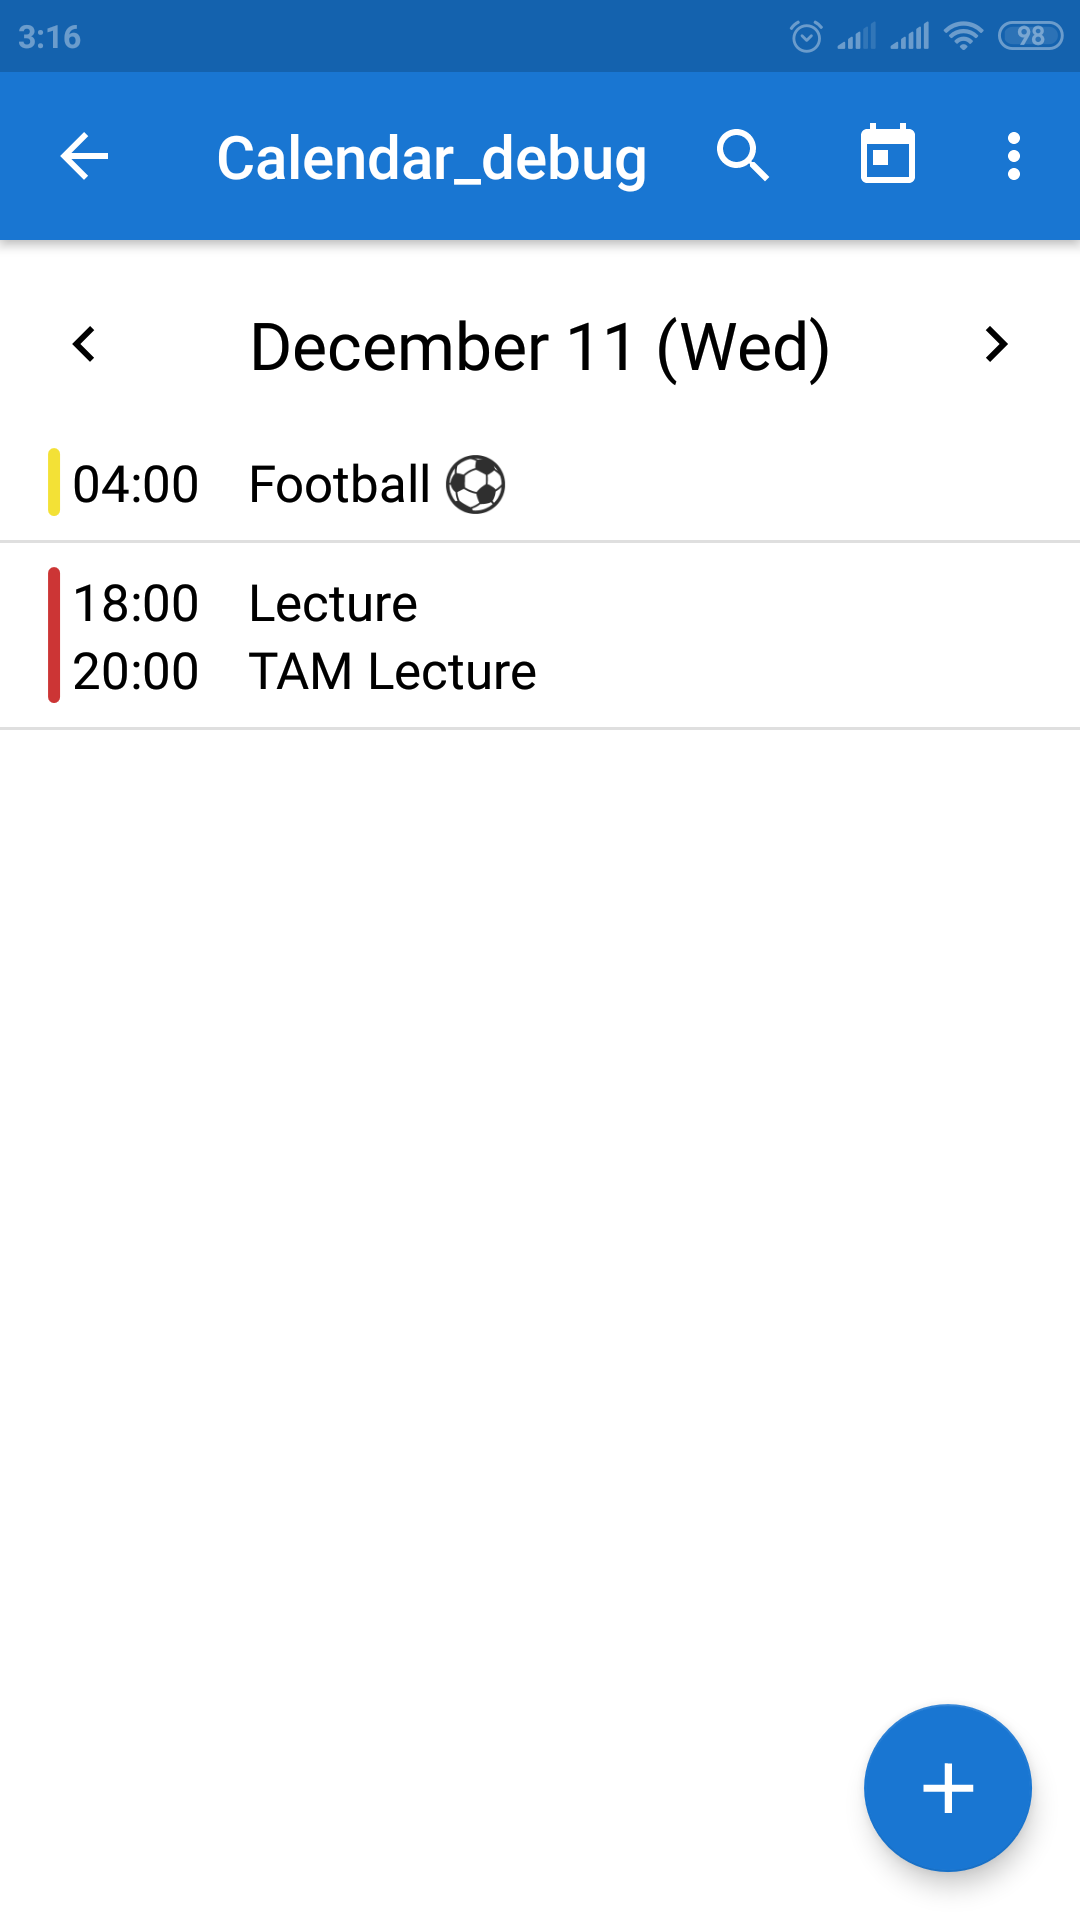
\includegraphics[width=10.5em, frame]{img/calendar_day.png}
			\caption{A~daily view}
		\end{subfigure}
%
		\begin{subfigure}{.24 \textwidth}
			\centering
			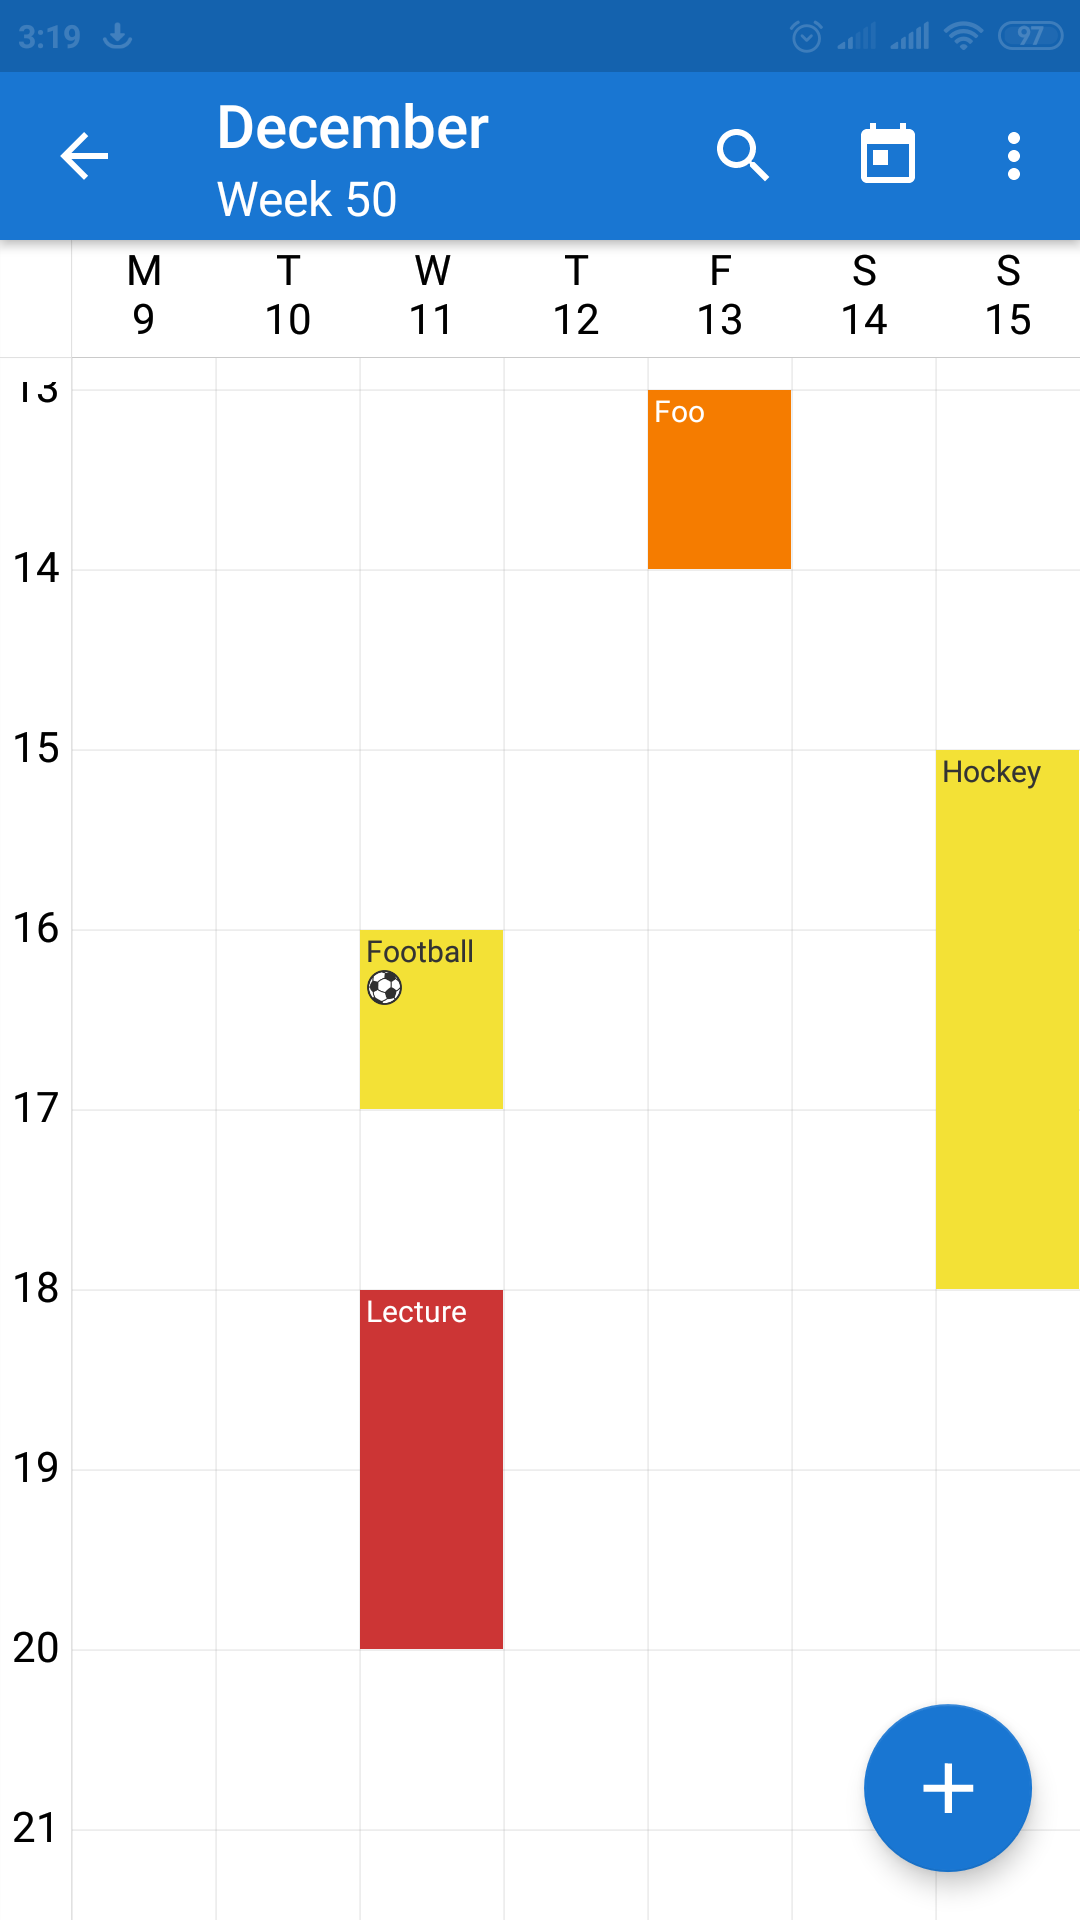
\includegraphics[width=10.5em, frame]{img/calendar_week.png}
			\caption{A~weekly view}
		\end{subfigure}
%
		\begin{subfigure}{.24 \textwidth}
			\centering
			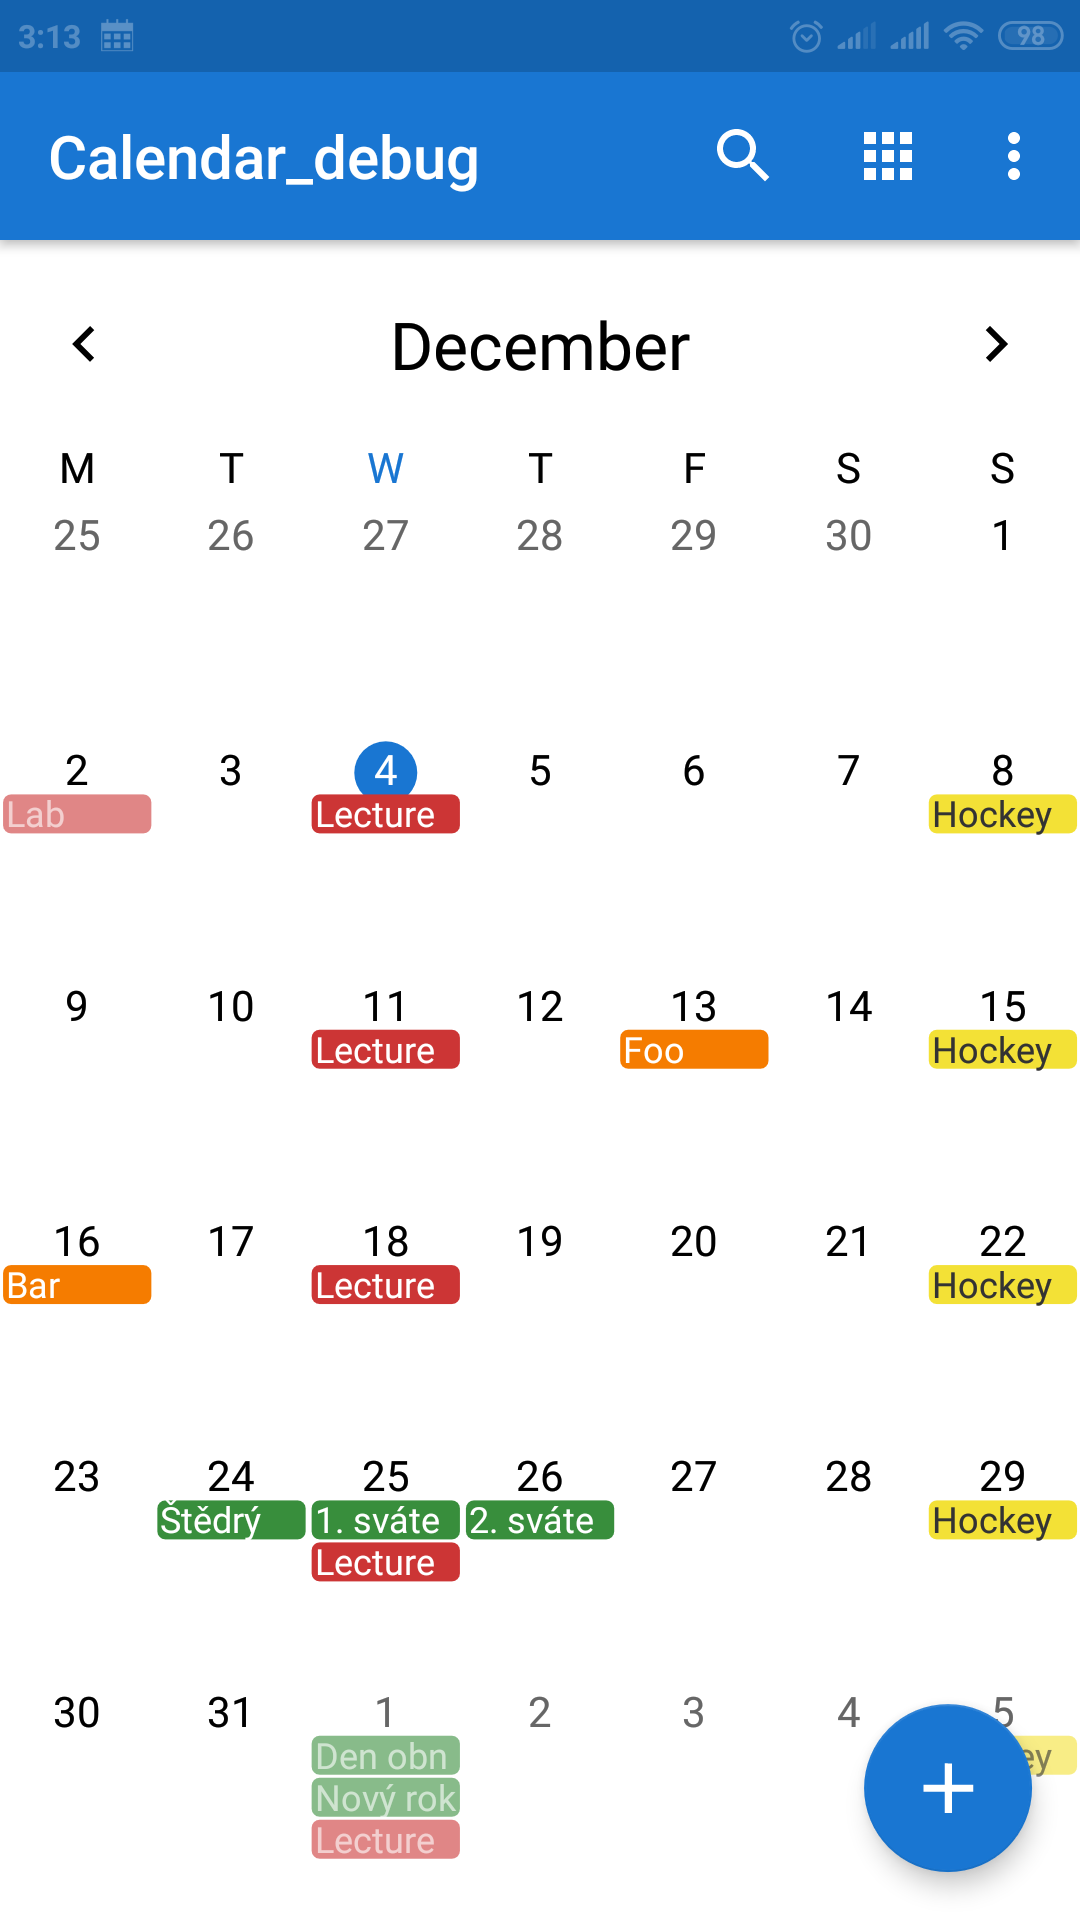
\includegraphics[width=10.5em, frame]{img/calendar_month.png}
			\caption{A~monthly view}
		\end{subfigure}
%
		\begin{subfigure}{.24 \textwidth}
			\centering
			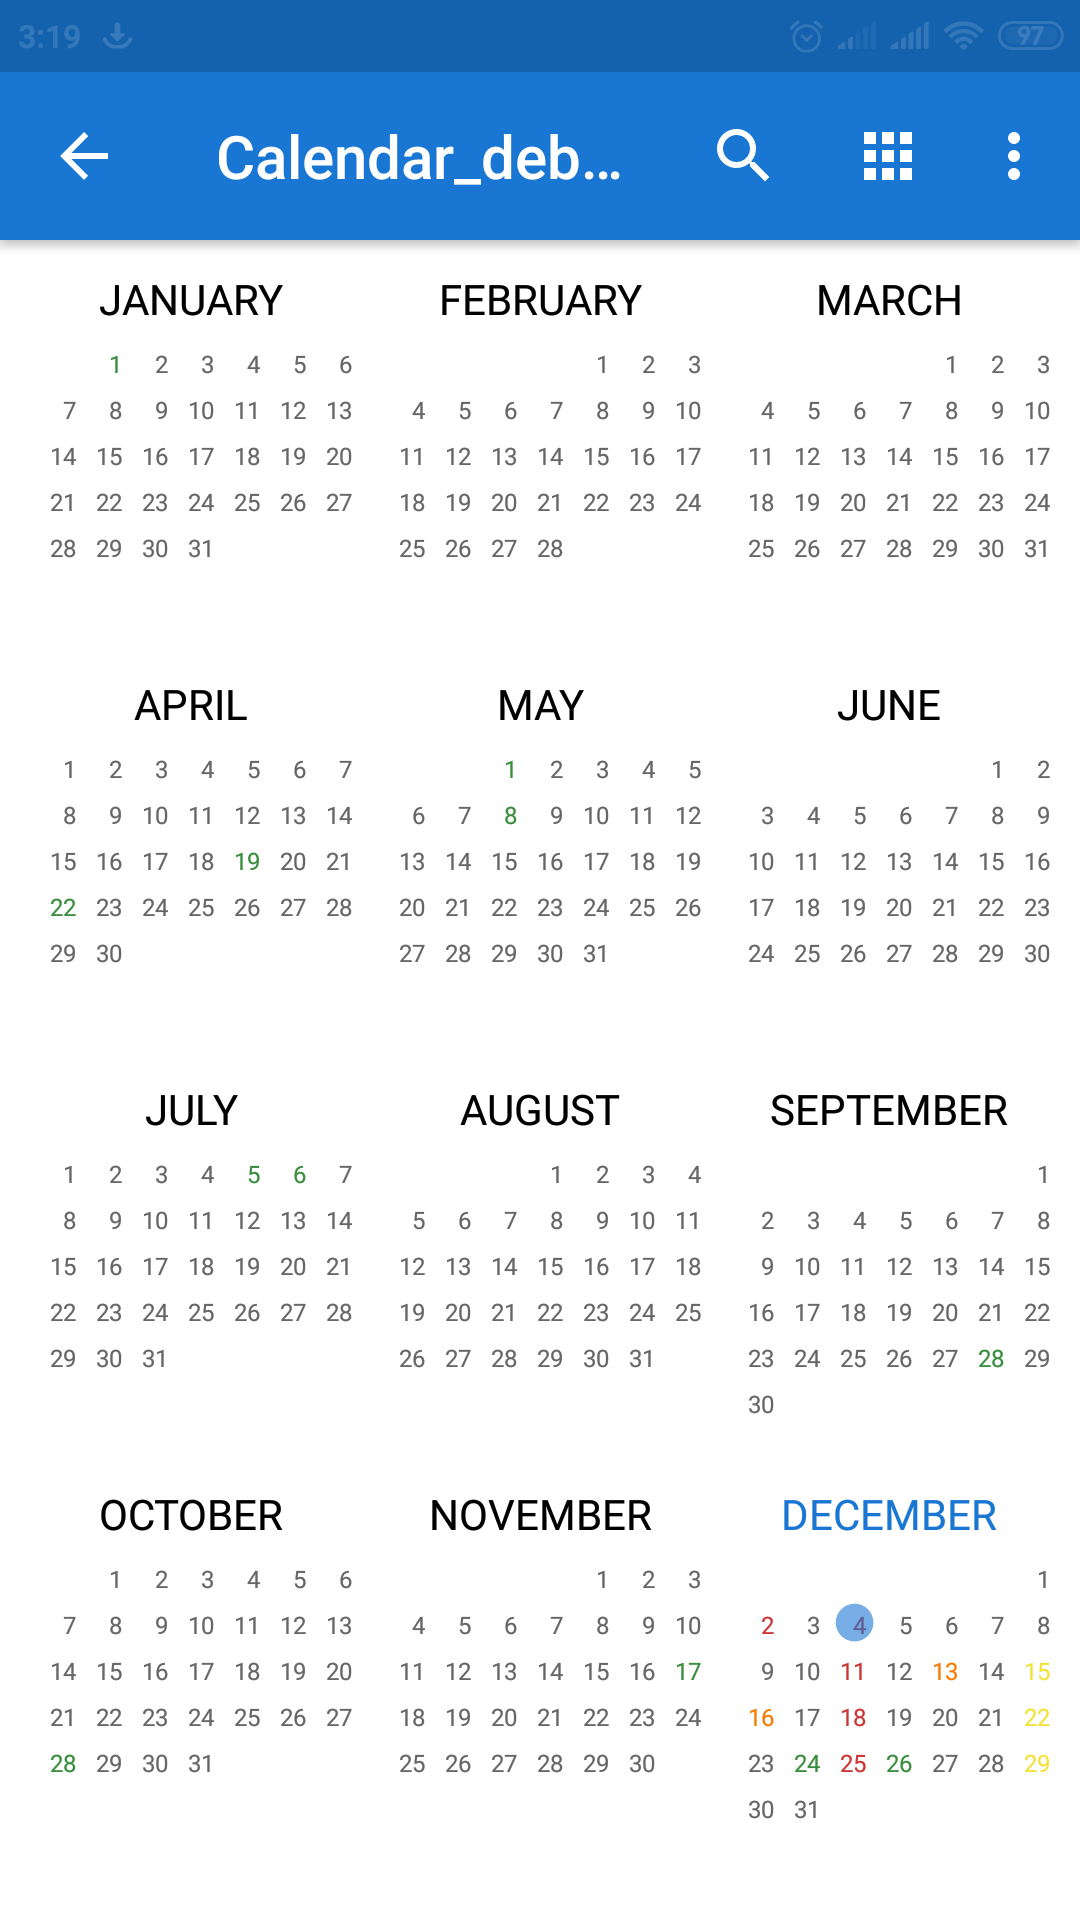
\includegraphics[width=10.5em, frame]{img/calendar_year.png}
			\caption{A~yearly view}
		\end{subfigure}

		\caption{Different views of the main screen of the application}
		\label{fig:calendar-views}
	\end{figure}

	Figure~\ref{fig:calendar-event-list} demonstrates another special
	calendar view. It is a~list of all days that hold some events. In
	other words, it is a~list of all created events.

	\begin{figure}[ht]
		\centering

		\begin{minipage}{.45\textwidth}
			\centering
			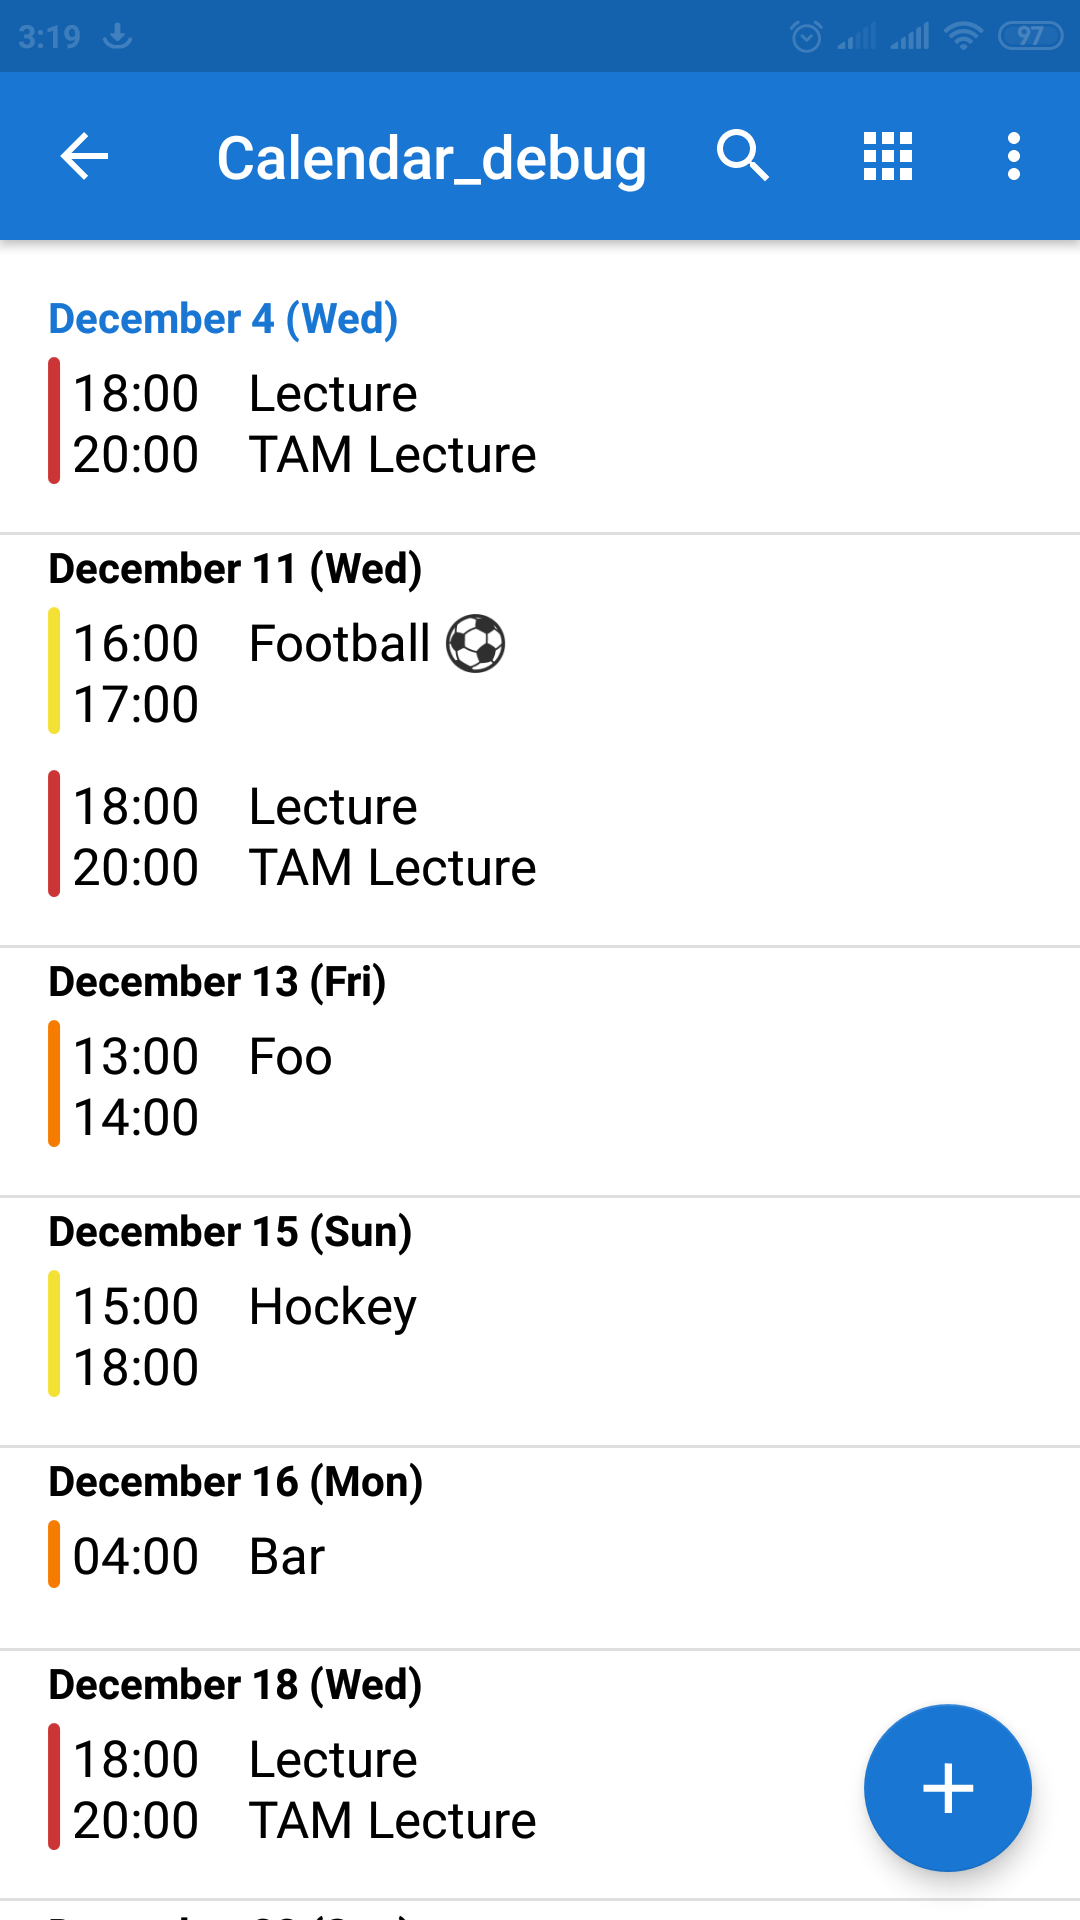
\includegraphics[width=10.5em, frame]{img/calendar_event_list.png}
			\caption{An event list view}
			\label{fig:calendar-event-list}
		\end{minipage}
	%
		\begin{minipage}{.53\textwidth}
			\centering

			\begin{subfigure}{.49 \textwidth}
				\centering
				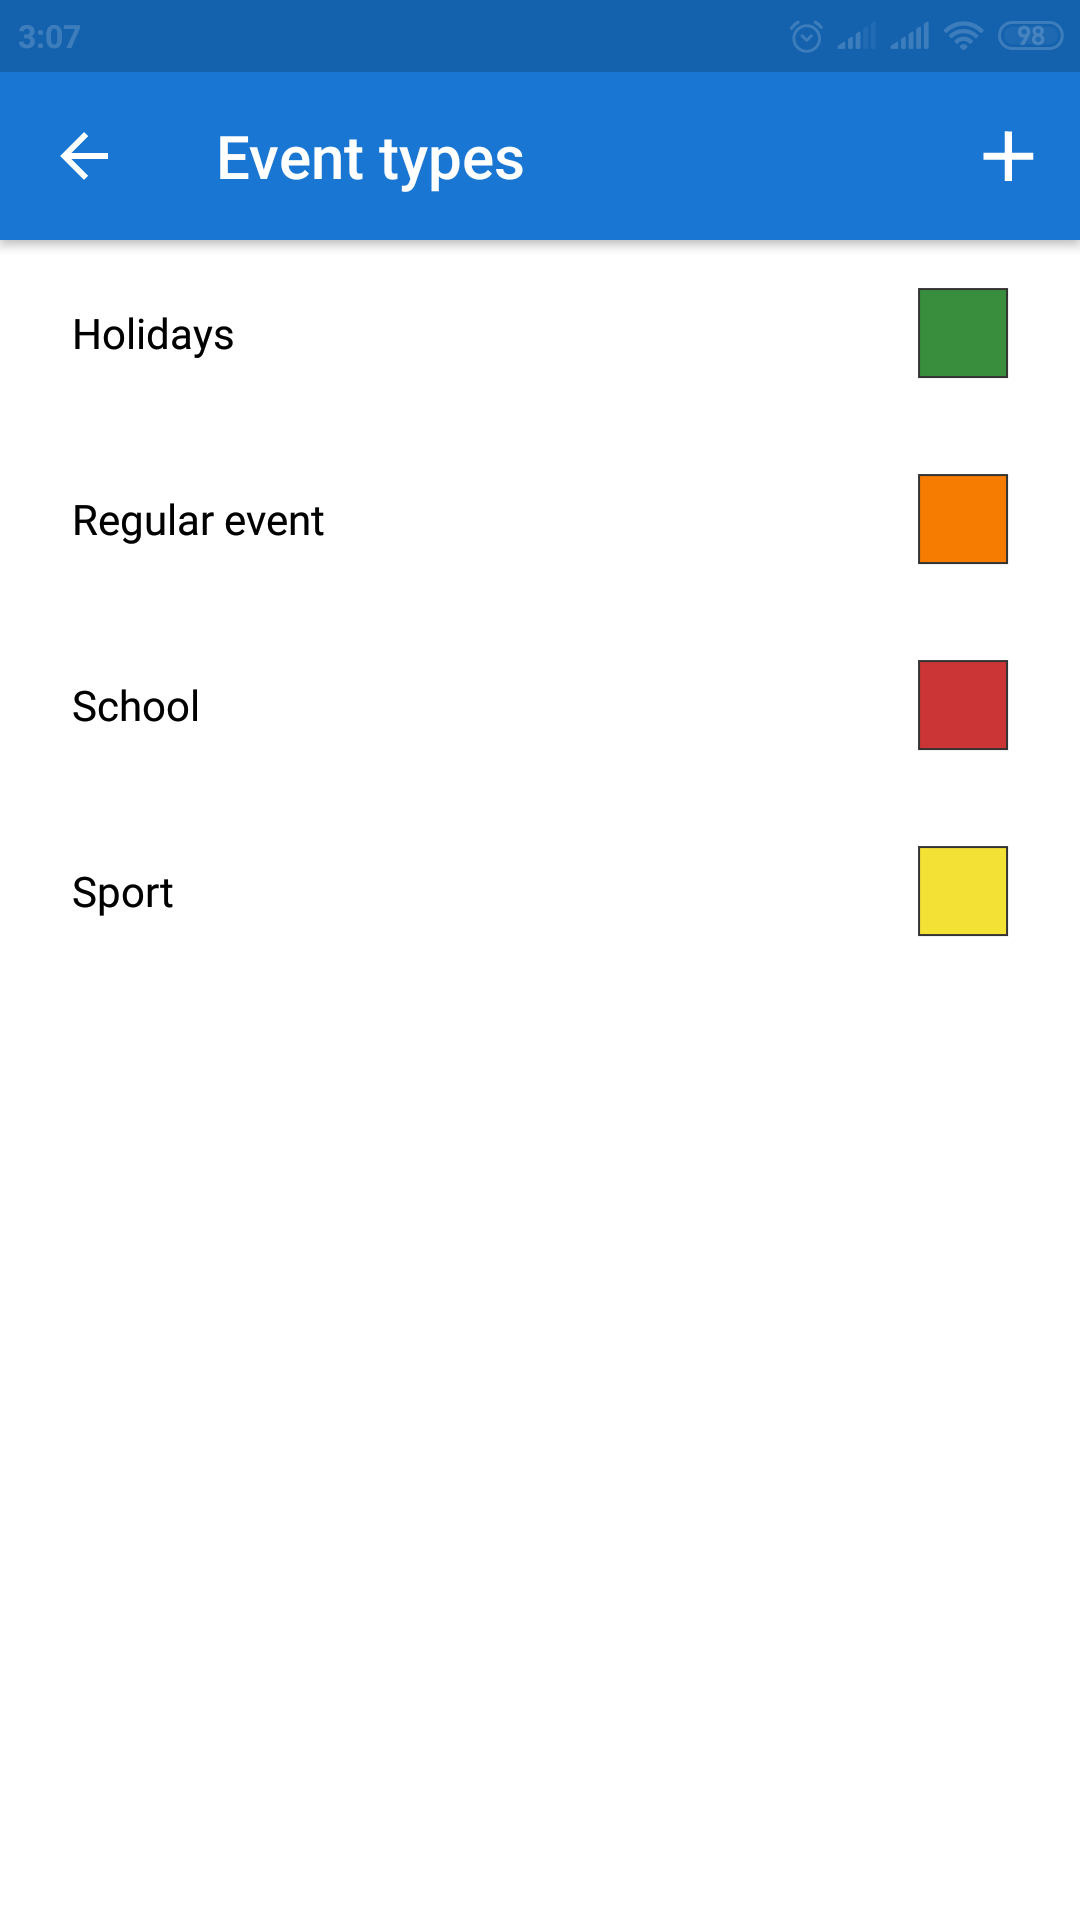
\includegraphics[width=10.5em, frame]{img/event_types.png}
				\caption{A~list of event types}
			\end{subfigure}
	%
			\begin{subfigure}{.49 \textwidth}
				\centering
				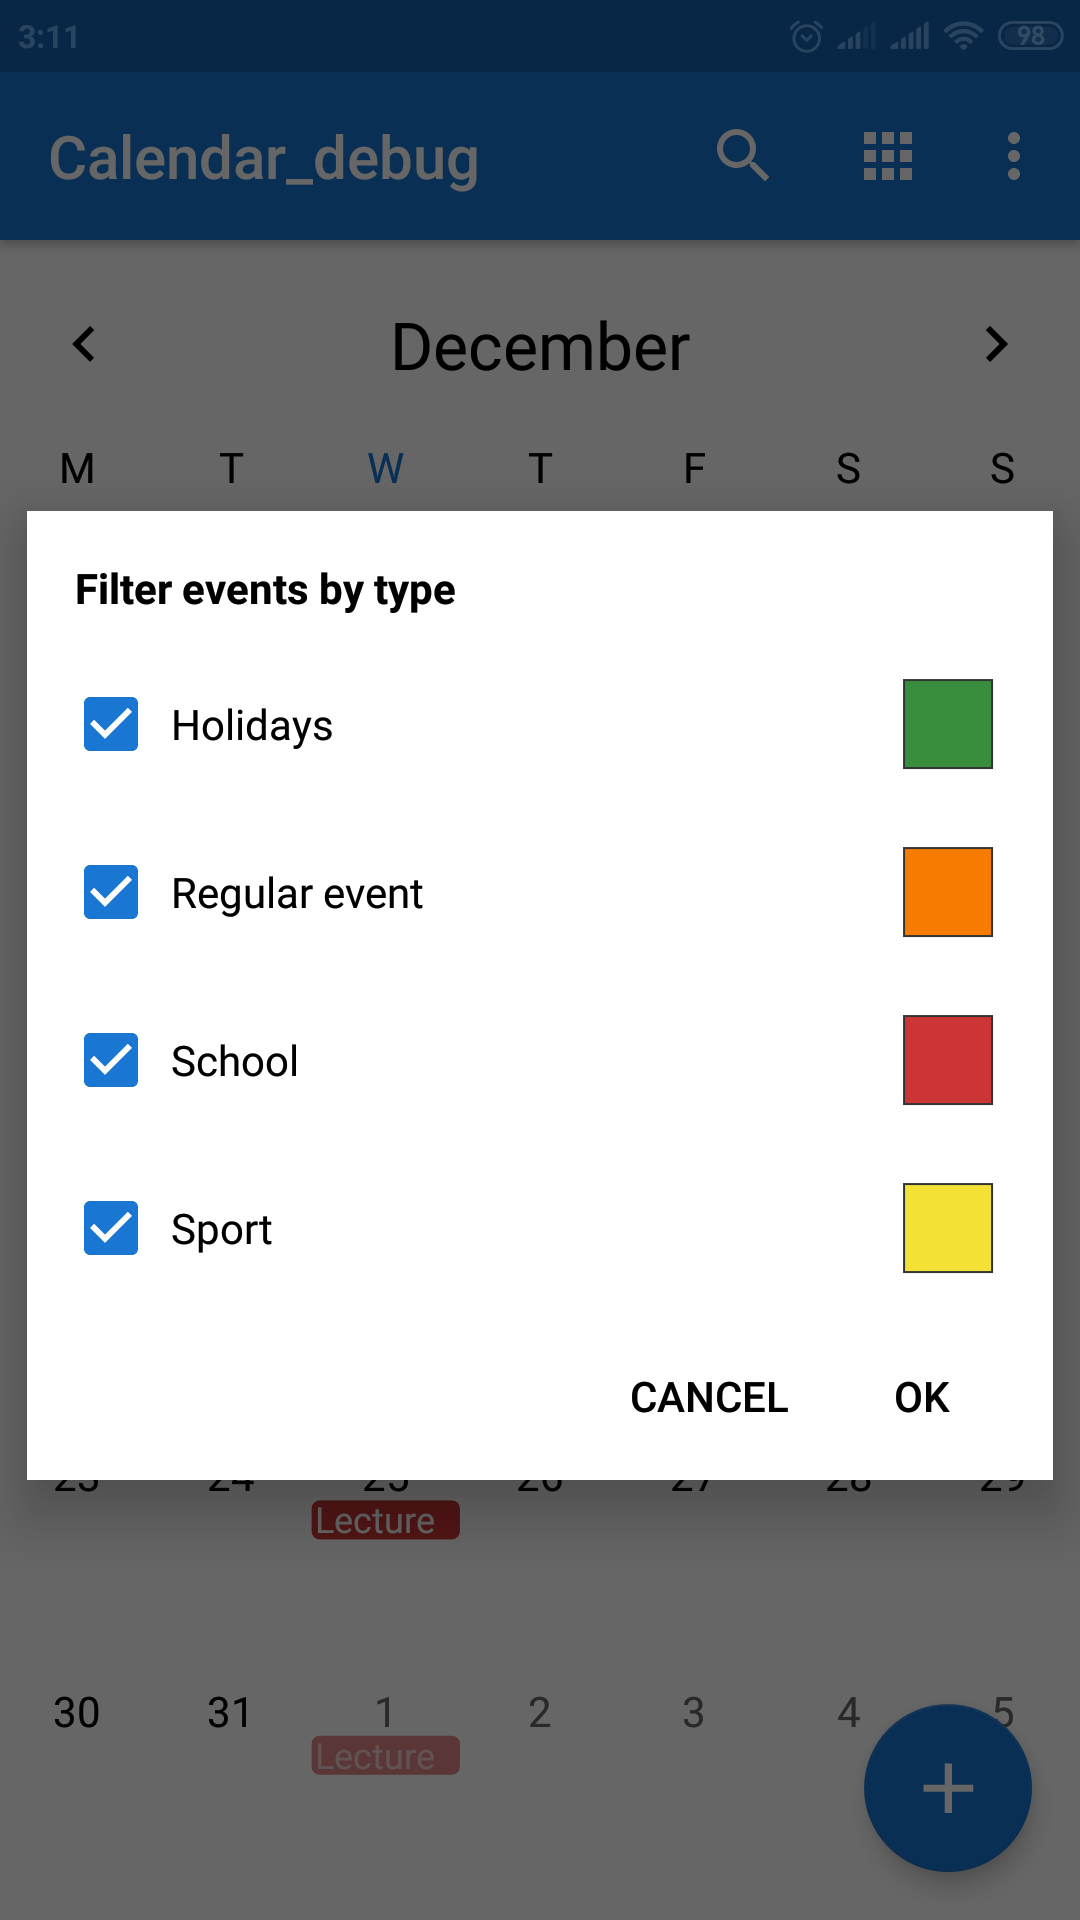
\includegraphics[width=10.5em, frame]{img/filter_events.png}
				\caption{Filtering events by its type}
			\end{subfigure}

			\caption{Event types}
			\label{fig:event-types}
		\end{minipage}
	\end{figure}

	In Figure~\ref{fig:event-types}, there can be seen work with
	\emph{events types}. Several types can be created and assigned to
	particular events. Event types are distinguished by their names
	and colours. Afterwards, events in the calendar can by filtered
	be these types.

	New events can be created using a~simple form, as it is shown in
	Figure~\ref{fig:add-event}. In this form, there can be specified
	a~name of the event, description, its location (the location can
	be easily opened in a~maps application), time and duration,
	reminders, repetition of the event, and its type. Default values
	of these fields may be defined in settings.

	\begin{figure}[H]
		\centering

		\begin{minipage}{.24 \textwidth}
			\centering
			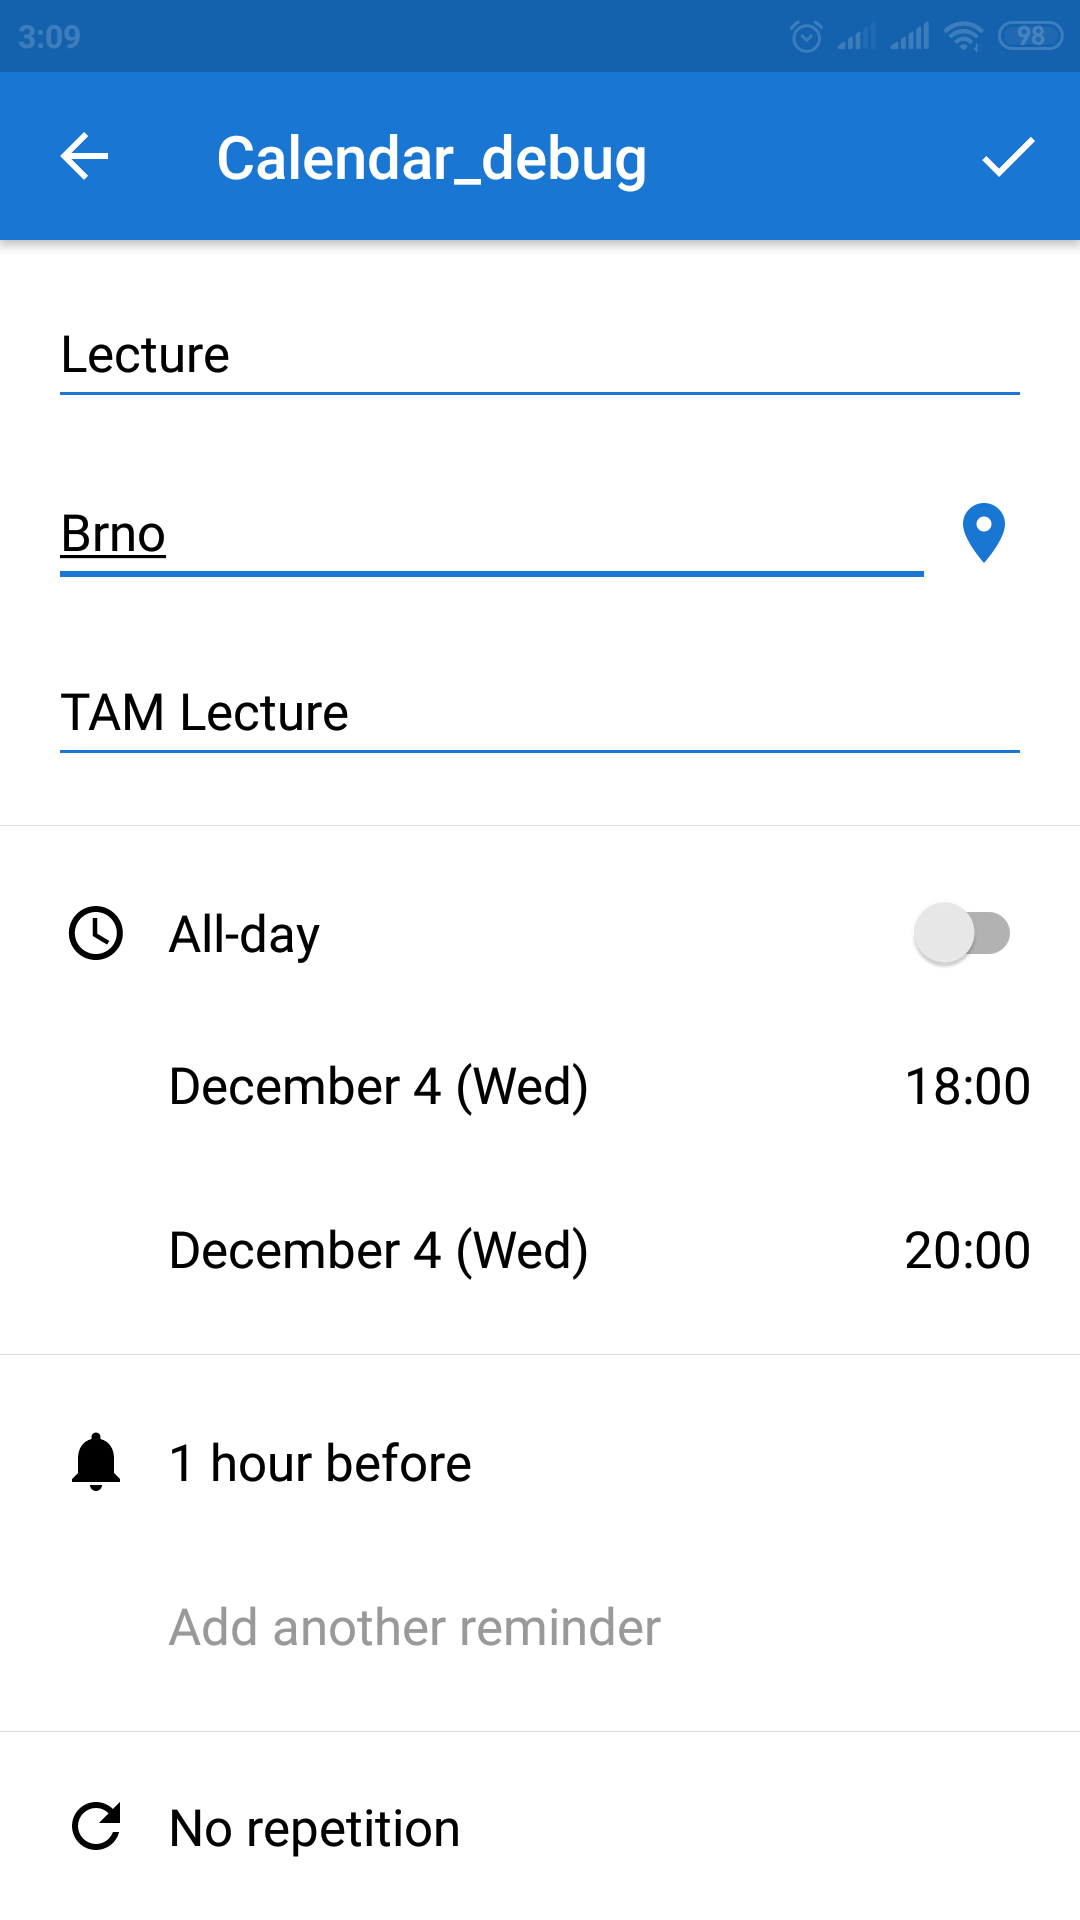
\includegraphics[width=10.5em, frame]{img/add_event.png}
			\caption{Adding a~new event}
			\label{fig:add-event}
		\end{minipage}
%
		\begin{minipage}{.74 \textwidth}
			\centering

			\begin{subfigure}{.32 \textwidth}
				\centering
				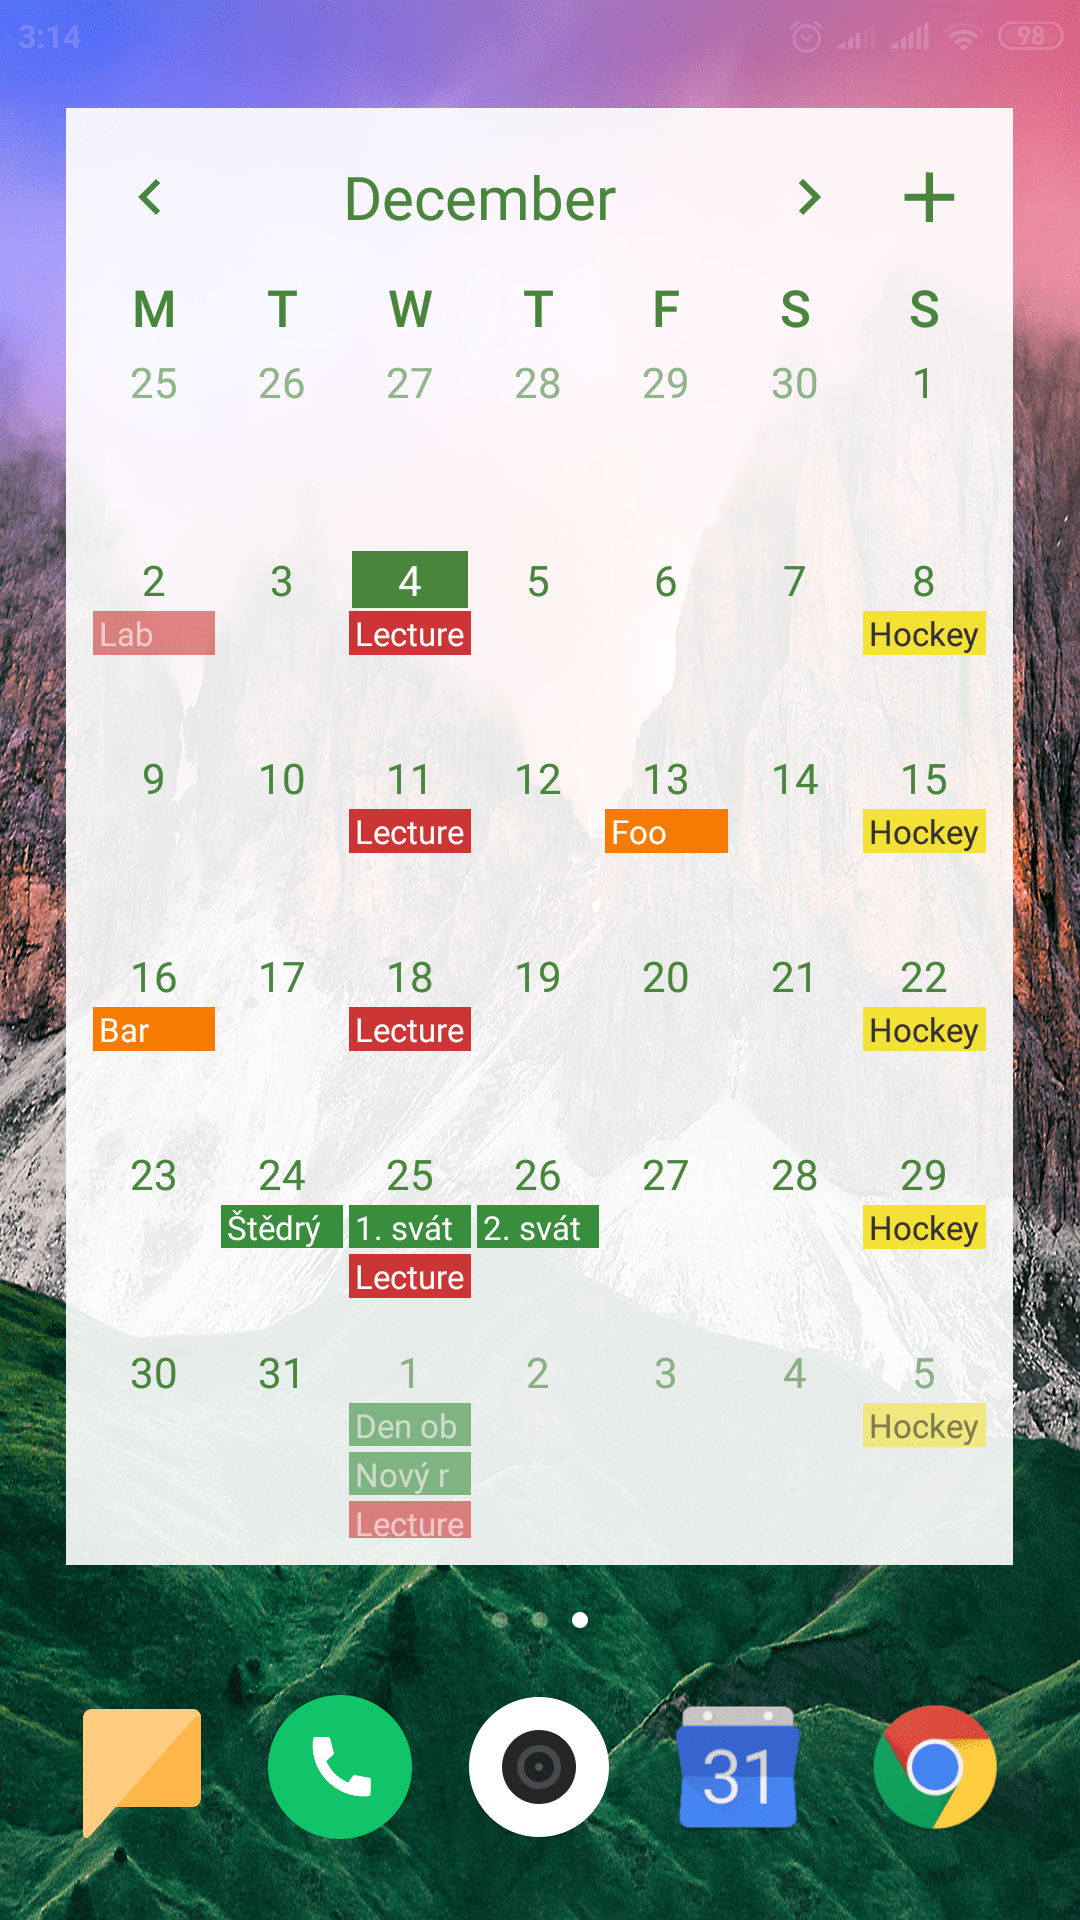
\includegraphics[width=10em, frame]{img/widget_month.png}
				\caption{A~widget with a~monthly view calendar}
			\end{subfigure}
	%
			\begin{subfigure}{.32 \textwidth}
				\centering
				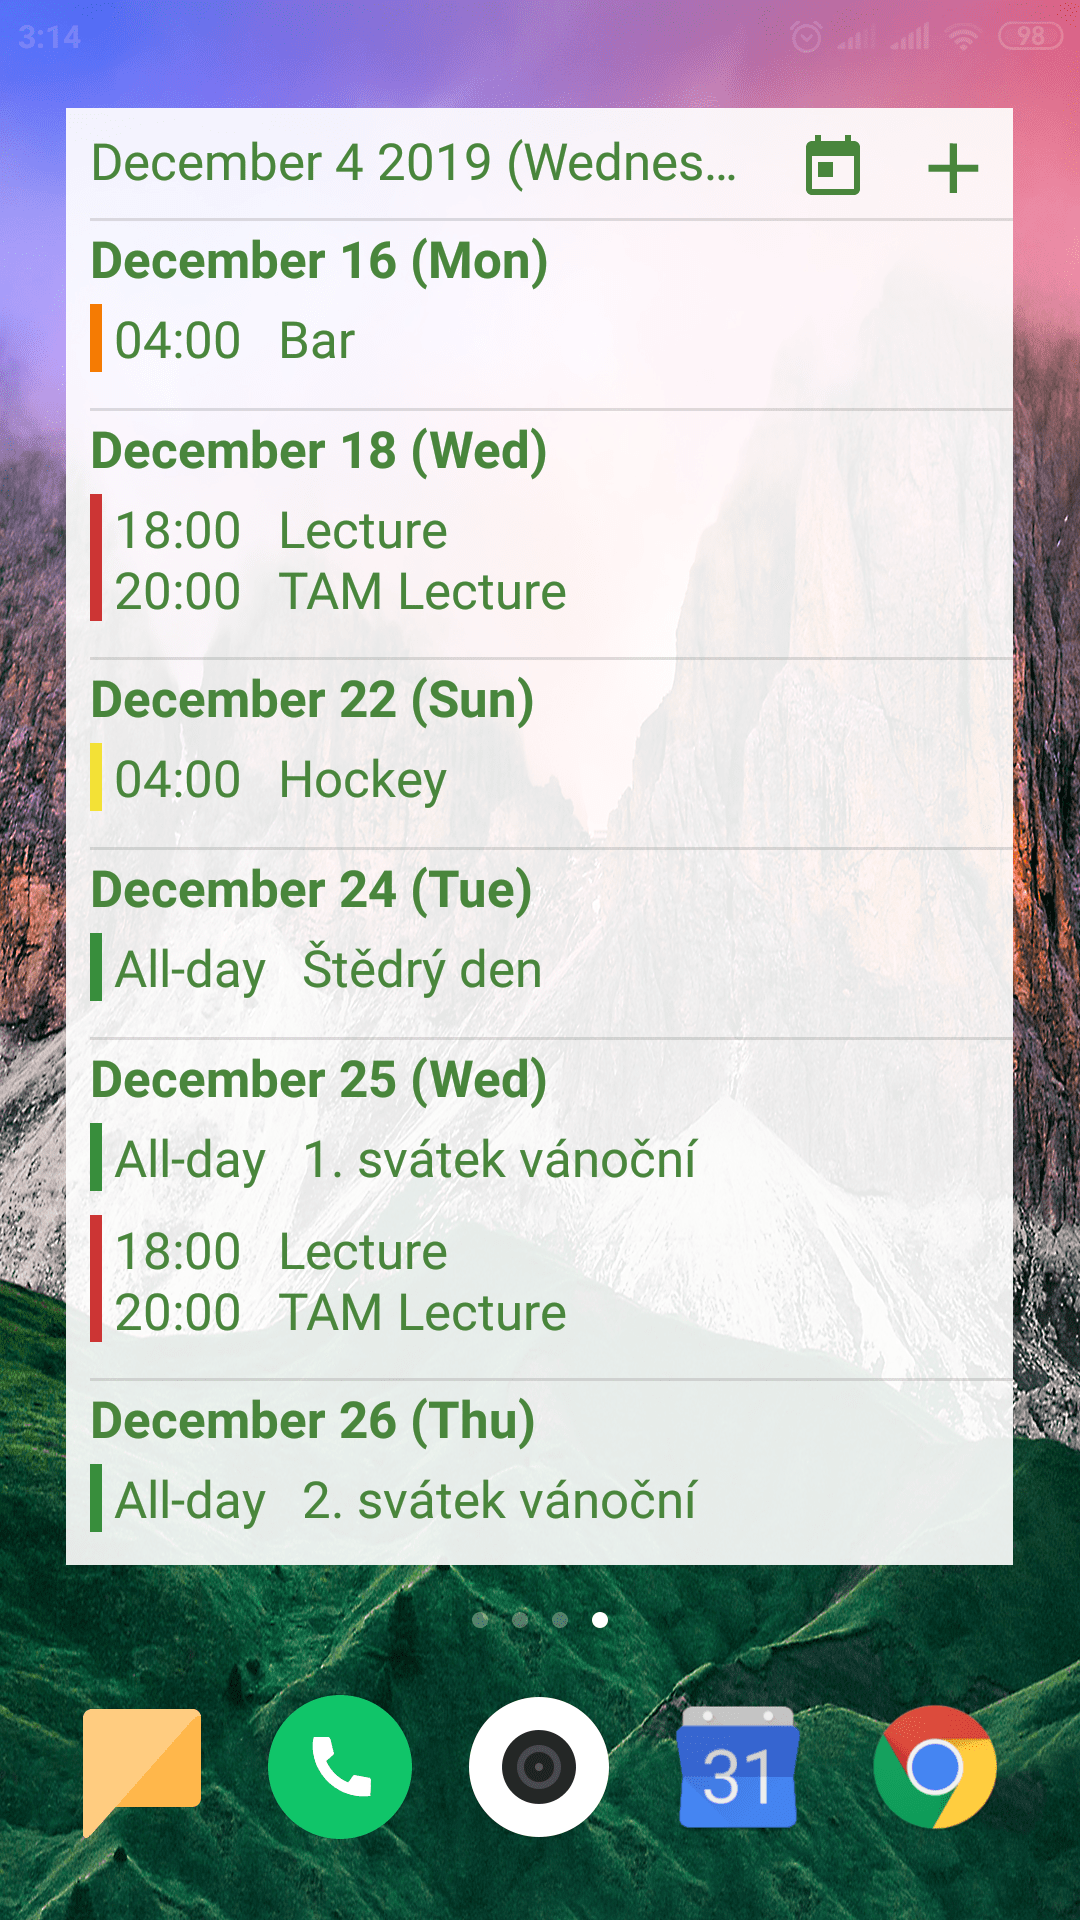
\includegraphics[width=10em, frame]{img/widget_event_list.png}
				\caption{A~widget with an event list view}
			\end{subfigure}
	%
			\begin{subfigure}{.32 \textwidth}
				\centering
				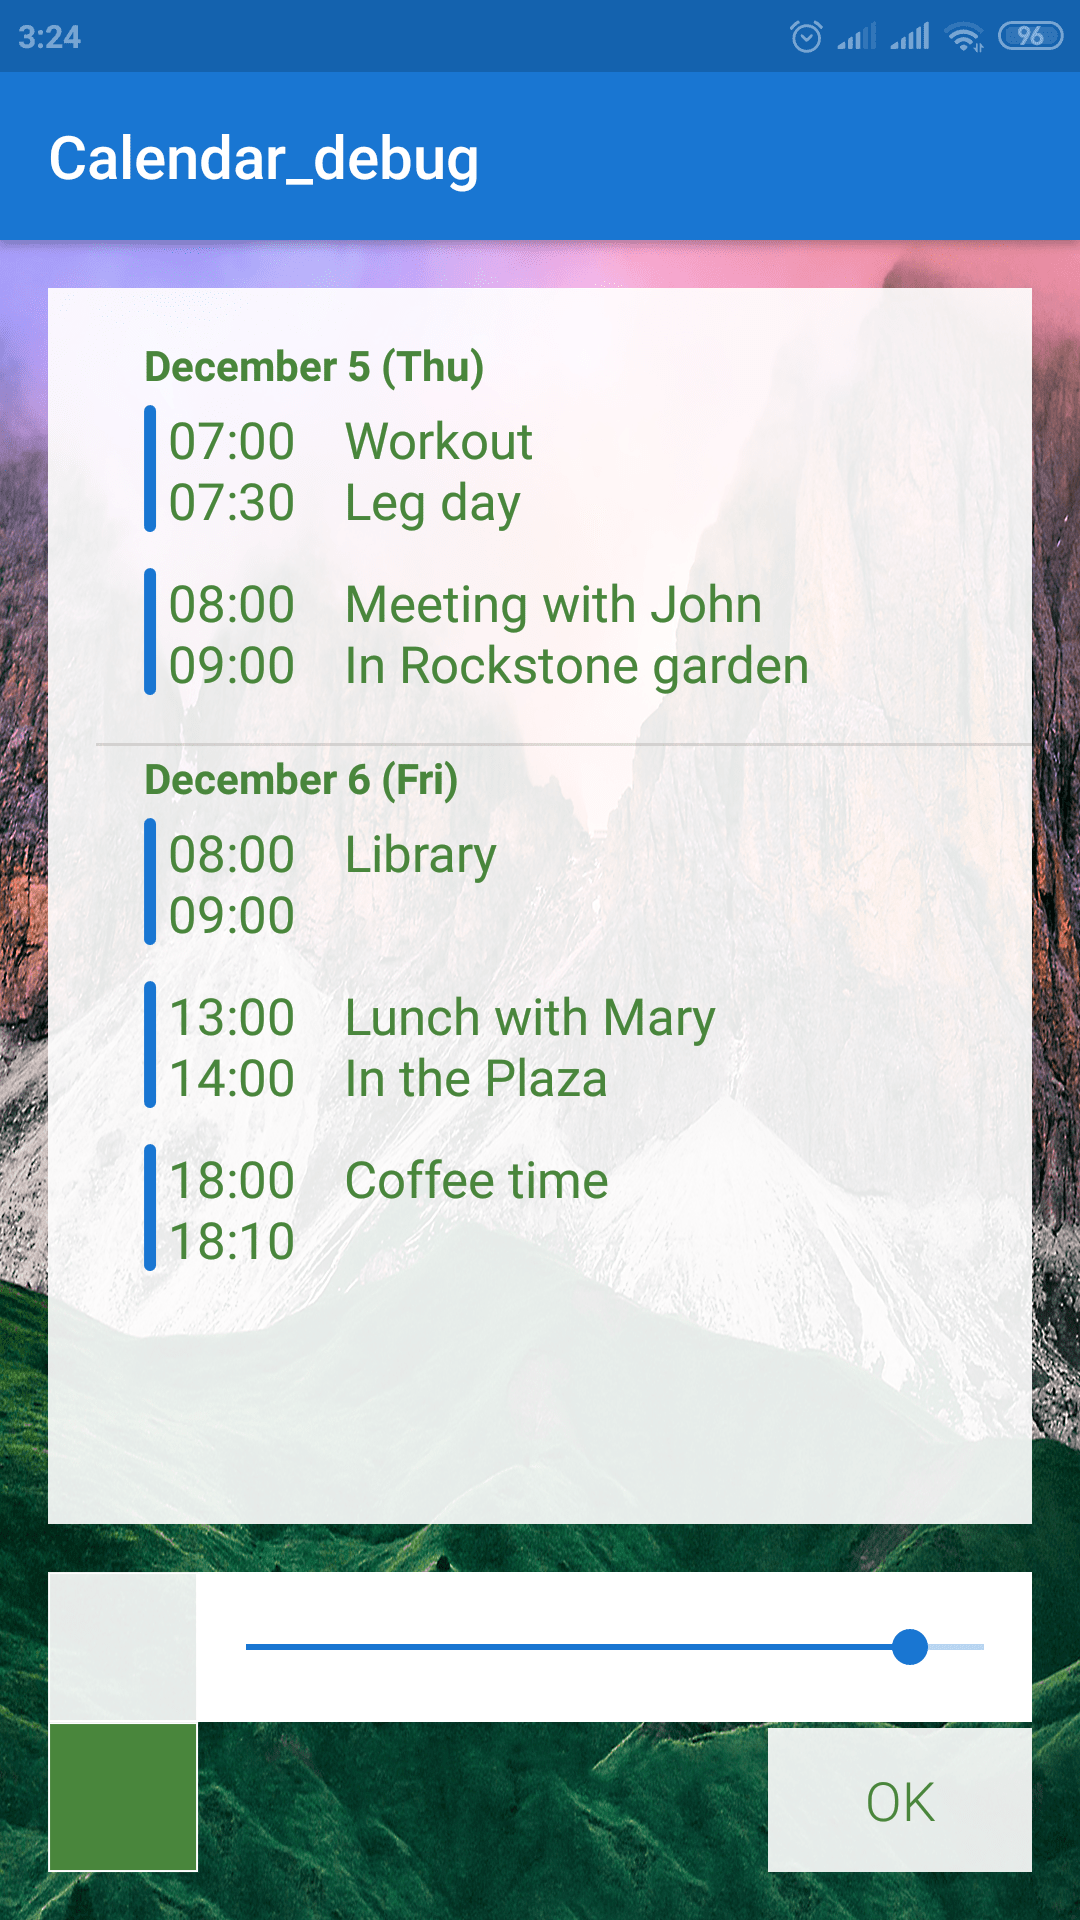
\includegraphics[width=10em, frame]{img/widget_customise.png}
				\caption{Customisation of widget colours}
			\end{subfigure}

			\caption{Desktop widgets}
			\label{fig:widgets}
		\end{minipage}
	\end{figure}

	Figure~\ref{fig:widgets} demonstrates available \emph{desktop widgets} 
	and options of their customisation. There is one widget with a~monthly
	view and another one with a~list of events. Both colours of the text
	and colours of the background can be modified. Transparency of the
	background can be modified as well.

	Not only colours of widgets can be customised but other colours in
	the application may be customised too, as it is shown in
	Figure~\ref{fig:colours}. In this Figure, there also can be seen two
	variants of colour pickers.

	\begin{figure}[ht]
		\centering

		\begin{subfigure}{.32 \textwidth}
			\centering
			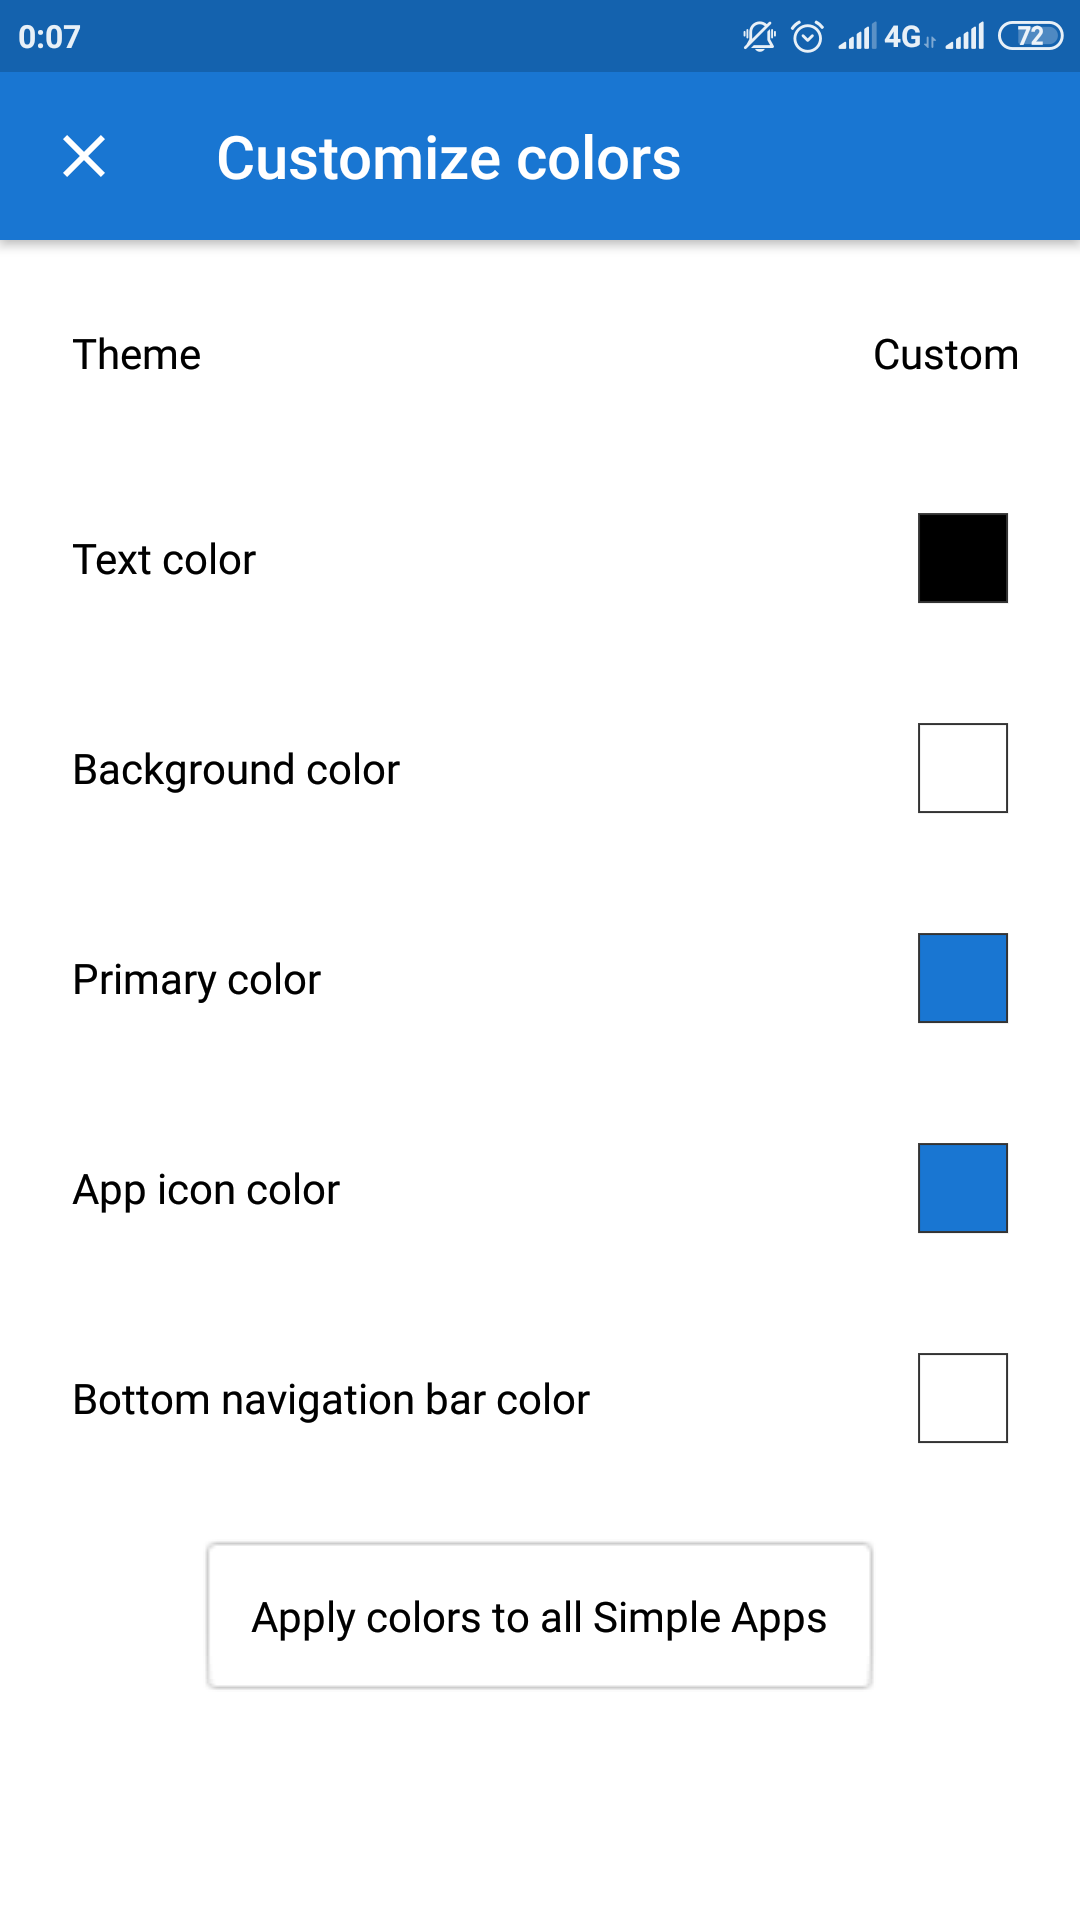
\includegraphics[width=10.5em, frame]{img/custom_colours.png}
			\caption{Options of colours customisation}
		\end{subfigure}
%
		\begin{subfigure}{.32 \textwidth}
			\centering
			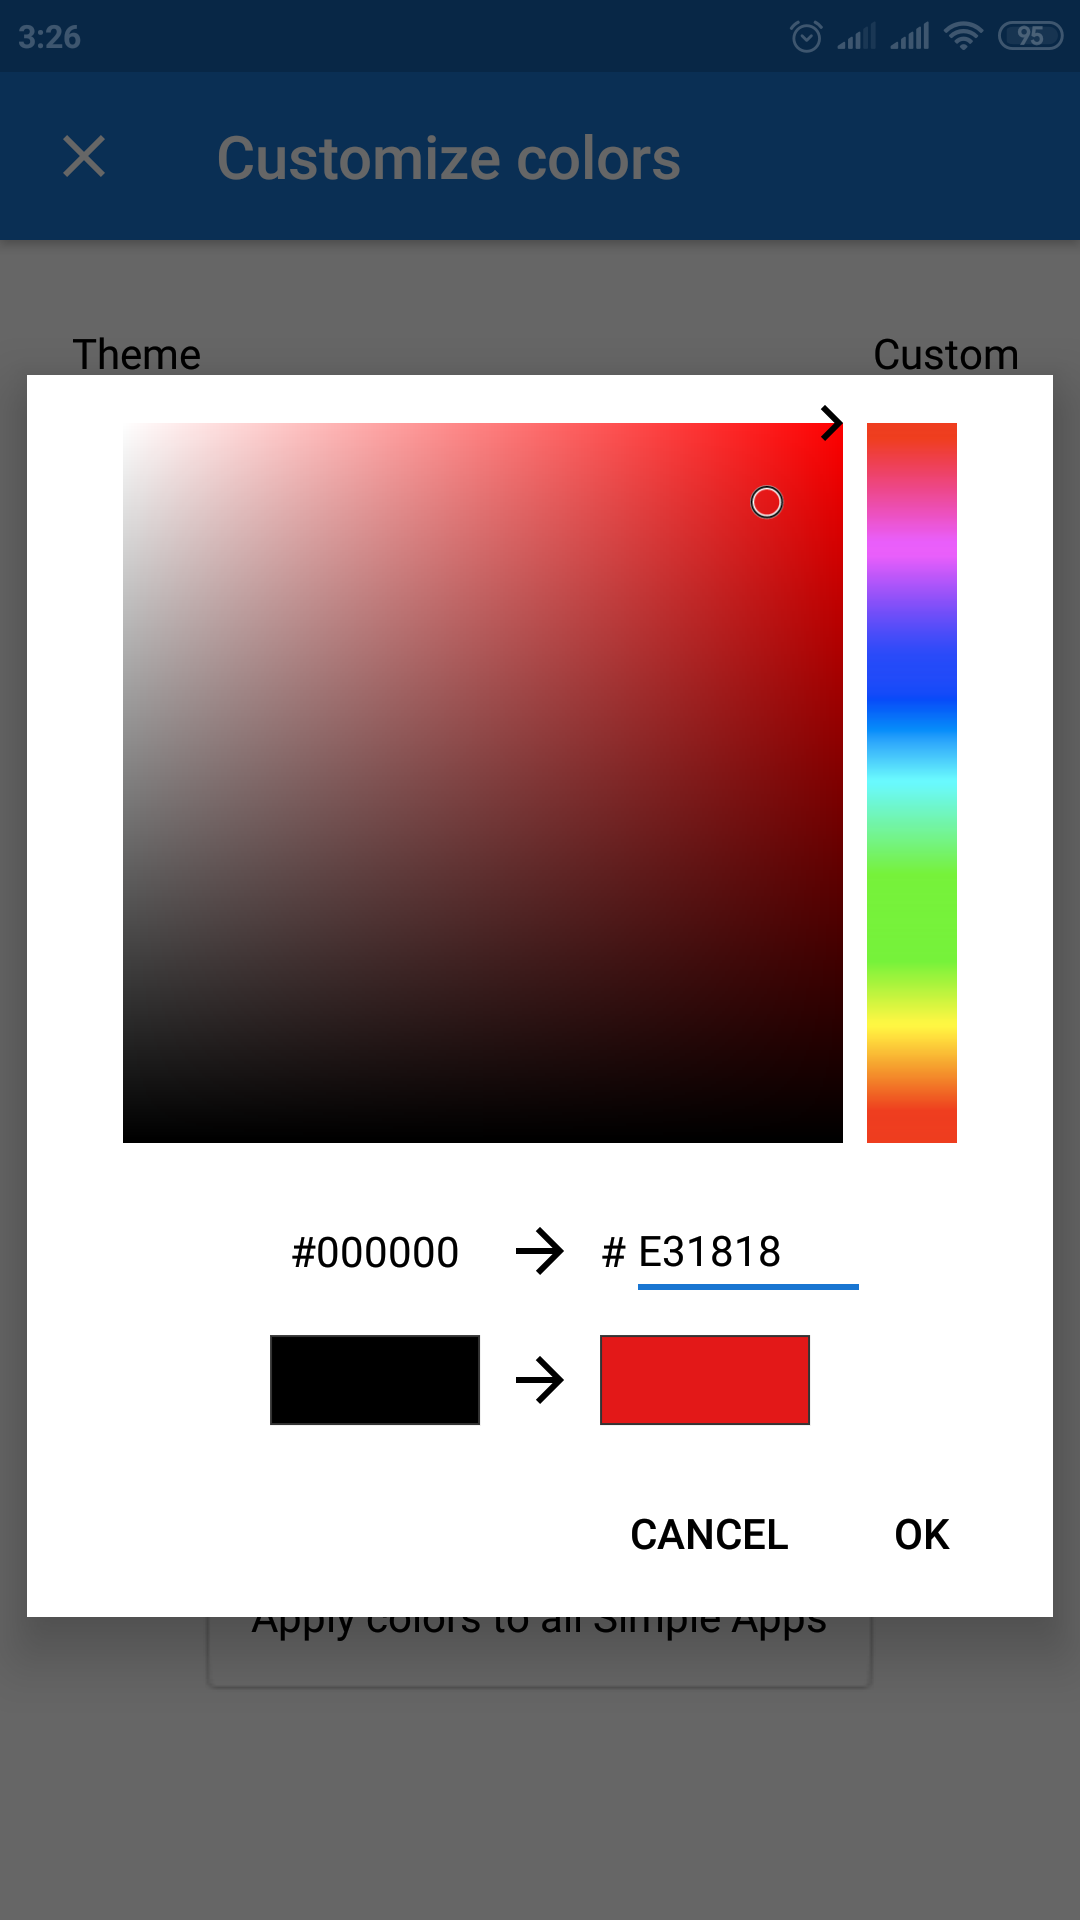
\includegraphics[width=10.5em, frame]{img/color_picker_1.png}
			\caption{The colour picker 1}
		\end{subfigure}
%
		\begin{subfigure}{.32 \textwidth}
			\centering
			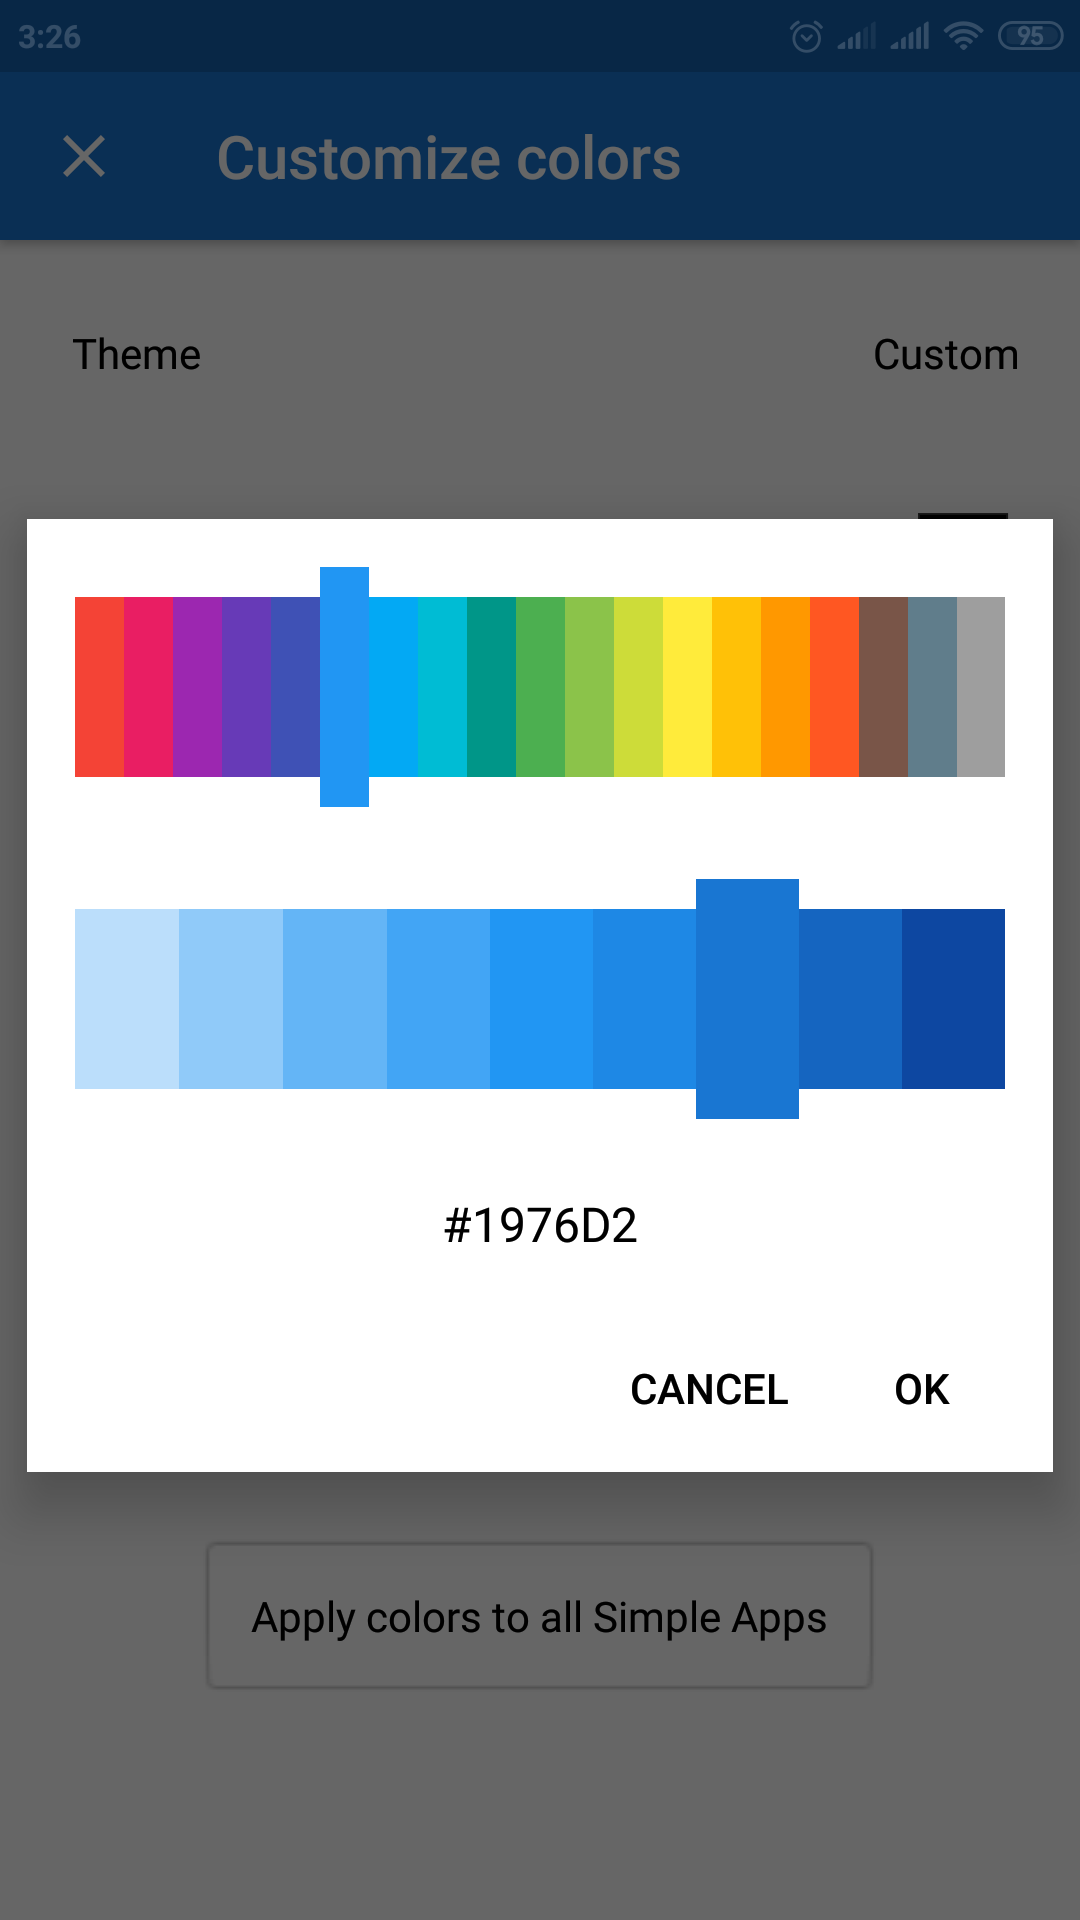
\includegraphics[width=10.5em, frame]{img/color_picker_2.png}
			\caption{The colour picker 2}
		\end{subfigure}

		\caption{Colours customisation}
		\label{fig:colours}
	\end{figure}


	\section{
		\texorpdfstring{
			History of the Application\protect\footnote{%
				A~\textbf{changelog} of the Simple Calendar application\,--\,%
				\url{https://github.com/SimpleMobileTools/Simple-Calendar/blob/master/CHANGELOG.md}.
			}
		}{History of the Application}
	}
	\label{sec:history}

	As it was already mentioned, the application is open-source, so
	any version of the application can be downloaded, compiled, and
	installed. A~few \emph{major versions} has been installed and analysed.

	Since the first release of the application up to version 2.0.0,
	several significant changes were made. A~widget for a~list of
	events was added and widgets can be resized. Further, it was
	added a~yearly calendar view, dark theme, event notifications,
	repetitive options for events, and there is a~new confirmation
	dialogue before deleting events.

	In version 2.x.x, the following changes were made. More colour
	themes were added, colours can be customised in more detail,
	and the  colour picker was reworked. Events can be imported and 
	exported to/from ICS files and CalDAV synchronisation was implemented.
	Options of adding reminders and options of setting repeatable events
	were significantly extended. A~weekly view and event types were
	added. There are new features that allow one to automatically
	import holidays of selected countries and contact's birthdays
	and anniversaries.

	In version 3.x.x, mostly bug fixes and performance issues
	were handled. Moreover, a~daily calendar view was added and
	searching of events was implemented.

	In version 4.x.x, there are not any interesting new features.
	Mainly, some other bug fixes were made and some new translations
	were added.

	In version 5.1.3, free version of the application was marked
	as deprecated and in version 6.0.0, professional version has been
	released. Version 6 is currently the latest version. In this version,
	there is allowed to import and export settings of the application.
	And several other glitches were fixed.


	\section{Strengths, Weaknesses, and Conclusion}
	\label{sec:conclusion}

	Android application Simple Calendar has been analysed and it has
	been discussed its design, user interface, and history of the
	development.

	The best thing about the application\,---\,the reason why quite many
	people use this application\,---\,is that it is a~\emph{lightweight
	minimalist variant} to a~classic calendar application. The usage is 
	really simple, \emph{straight-forward} and it is \emph{intuitive}. 
	Another good thing is that it is \emph{highly customisable}, there are 
	no \emph{unnecessary permissions} required, and there is no need for
	internet connection. Optionally, there are possibilities to synchronise
	the calendar with other applications or devices if it is demanded. The
	application has many translations and it has a~quite handsome and 
	\emph{decent design}. Moreover, the application is live and open-source.

	The \emph{week point} of the application is that professional up to date
	version is not for free. This can discourage the users because there
	are available plenty of other free applications of a~similar kind,
	even so, this one is fairly cheap. There are many users that use,
	for example, Google Cloud Services or Microsoft Azure or something
	similar every day so they would likely prefer Google Calendar or
	Microsoft Outlook, etc. But undoubtedly, other users give way
	\emph{privacy} and \emph{simplicity} so this application might be 
	suitable for them.
\end{document}
